% !TeX spellcheck = en_GB

\section{Preface}\label{Preface}
In the software world, or more specific, the Java enterprise world, developers tend to abstract access to data in a way that components are interchangeable. A perfect example for such an abstraction is the usage of Object Relational Mappers (ORM). The database specifics are of lesser importance to the average developer compared to the actual business logic and the need for native SQL is brought down to a minimum. This makes the switch to a different relational database system (RDBMS) easier in the later stages of a product's life cycle.
\\\\
The Java Persistence API (JPA) went even further by providing a standardized API for ORMs. First conceived in 2006 as part of EJB 3.0 \footnote{JSR 220: Enterprise Java Beans 3.0, see~\cite{jsr_jpa1}} \footnote{Javaworld: Understanding JPA, Part 1, see~\cite{javaworld_jpa1}}, it is now the de-facto standard for Object Relational Mappers in Java. The developer doesn't need to know which specific ORM is used in the application, as all the database queries are written against the standardized query API and are therefore portable. This means that not only the database is interchangeable, but even the specific ORM, it is accessed by, is as well.
\\\\
However, this does not mean that all JPA implementations come with the same features. For example, some ship with additional modules to enhance their capabilities. A perfect example for this is the Hibernate Search API aimed at Hibernate ORM users.\footnote{Hibernate ORM project homepage, see~\cite{hibernate_orm}} \footnote{Hibernate Search project homepage, see~\cite{hibernate_search_homepage}}
\\\\

\pagebreak
\noindent
Nowadays, even small applications like online shops need enhanced search capabilities to let the user find more results for a given input.
This is not something a regular RDBMS excels at and Hibernate Search comes into use as shown in figure \ref{fig1}: It works atop the Hibernate ORM, a popular JPA implementation, and enables the developer to index the domain model for searching. It's not only a mapper from JPA entities to a search index, but also keeps the index up-to-date if something in the database changes.
\\
\begin{figure}[ht]
	\centering
	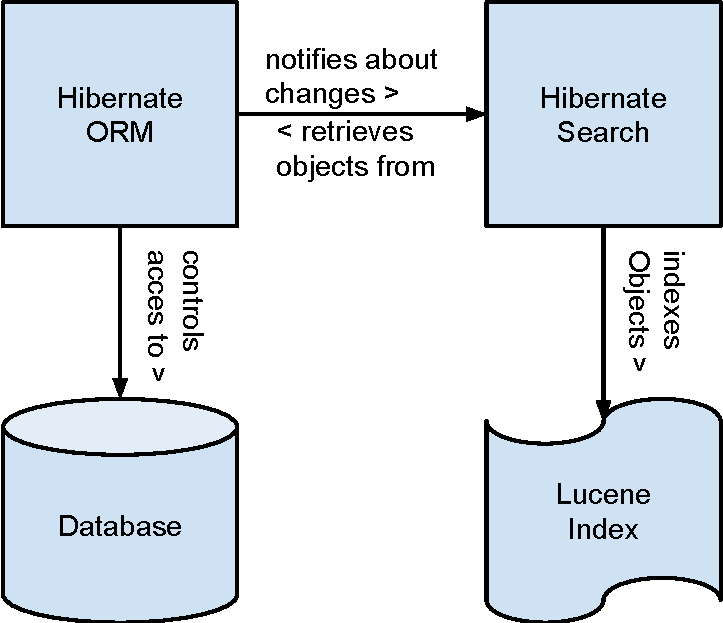
\includegraphics[scale=0.45]{images/hibernate_search_hibernate_schema.pdf}
	\caption{Hibernate Search with Hibernate ORM}
	\label{fig1}
\end{figure}
\\
Hibernate Search is based on the powerful Lucene search toolbox \footnote{sourcecode on Hibernate Search GitHub, see~\cite{hsearch_source_code_git}} \footnote{Hibernate Search FAQ, see~\cite{hibernate_search_faq}} and is a separate project in the Hibernate family. It aims to provide a JPA "feeling" in its API as it also incorporates a lot of JPA interfaces in its codebase. However, this does not mean that it is compatible with other JPA providers than Hibernate ORM (apart from Hibernate OGM, the NoSQL JPA mapper of the family) as the following figure \ref{fig2} shows.
\\\\
\begin{figure}[ht]
	\centering
	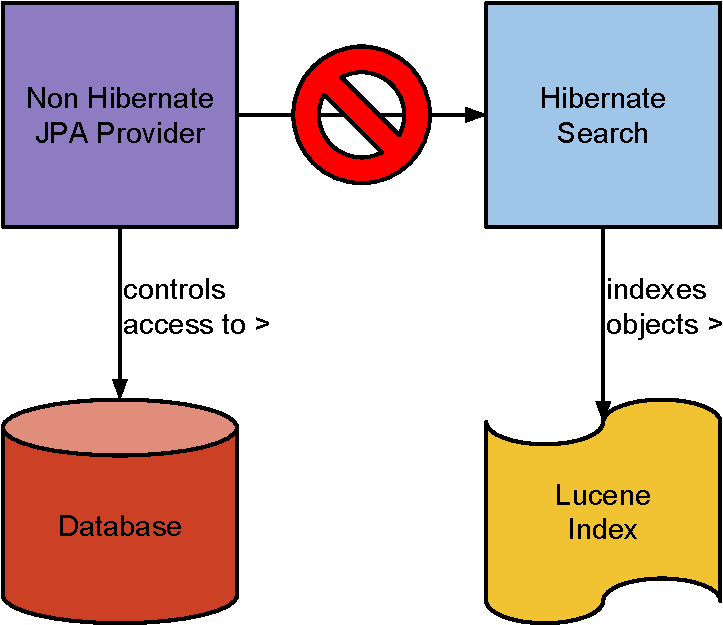
\includegraphics[scale=0.45]{images/hibernate_search_any_jpa_problem_schema.pdf}
	\caption{Hibernate Search's incompatibility with other JPA implementations}
	\label{fig2}
\end{figure}
\\
While using Hibernate Search obviously is beneficial for Hibernate ORM applications, not all developers can bind themselves to a specific JPA implementation in their application. For some, the ability to change implementations might be of strategic importance, for others it could just be sheer preference to use a different JPA implementation.

\noindent
Currently, developers that do not want to bind themselves to Hibernate ORM have to resort to using different full text search systems like native Lucene\footnote{official Lucene website, see~\cite{lucene_apache_org}}, ElasticSearch\footnote{ElasticSearch Java API, see~\cite{elasticsearch_java_api}} or Solr\footnote{Solr Java API, see~\cite{solr_java_api}}. While this is always a viable option, Hibernate Search would be a much better suit for some applications because of its design with a entity structure in mind combined with the automatic index updating feature, if it just were compatible with generic JPA.
\\\\
When investigating Hibernate Search's project structure
\footnote{Hibernate Search GitHub repository, see~\cite{hsearch_source_code_git}}, we can see that "hibernate-search-orm" is the only module apart from some server-integration modules that depends on any ORM logic. The modules that contain the indexing engine, the replication logic, alternative backends, etc. are completely independent from it. This means, that most of the codebase could be reused for a generic version of Hibernate Search.
\\\\
\noindent
Creating such a generic Hibernate Search is a better approach for a search API on top of JPA rather than rewriting a JPA binding from scratch. Hibernate Search could then act as the de-facto standard for fulltext search in the JPA world instead of having a competing API that would just do the same thing in a different style.
\\
\begin{figure}[ht]
	\centering
	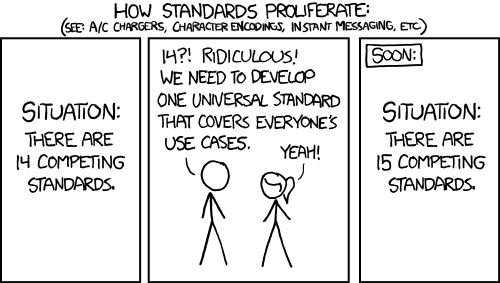
\includegraphics[scale=0.5]{images/competing_standards.png}
	\caption{xkcd.com on competing standards \protect\footnotemark}
	\label{xkcd_standards_fig}
\end{figure}
\footnotetext{xkcd comic \#927, see~\cite{xkcd_competing_standards_source}}
\\
This is why we will show how such a generic version can be built in this thesis. First, we will look at how Hibernate Search's engine can be reused. Then, we will write a standalone version of this engine and finally integrate it with generic JPA together with an automated index updating mechanism.

\pagebreak

\noindent
\textbf{Short overview of contents}:
\\\\
\noindent
In chapter \ref{Methods} we explain the methods we use to build Hibernate Search GenericJPA. In chapter \ref{Overview} we give an overview of the relevant technologies used in this thesis and give short introductions to several fulltext search engines and the reasoning behind Hibernate Search GenericJPA. In chapter \ref{Challenges} we introduce a small example project and explain the main challenges while developing Hibernate Search GenericJPA. In chapter \ref{standalone_chapter} we describe the standalone version of Hibernate Search. In chapter \ref{integration_jpa} we explain how the JPA integration of the standalone version is designed. In chapter \ref{automatic_indexing_chapter} we work out an automatic index updating mechanism for Hibernate Search GenericJPA. In chapter \ref{usage_chapter} we give a full explanation of how to use Hibernate Search GenericJPA using the example from chapter \ref{Challenges}. In chapter \ref{outlook} we give a summary of what we have achieved in this thesis and describe further steps.

\pagebreak

\pagebreak

\section{Methods} \label{Methods}

For the development of the generic version of Hibernate Search we use a combined approach of \textbf{top-down} \footnote{Top-down programming, Robert Strandh, see~\cite{top_down_strandh}} and \textbf{bottom-up} \footnote{Bottom-up programming, Robert Strandh, see~\cite{bottom_up_strandh}} software development: After dividing the project into submodules (top-down) we develop the "building blocks"  first and integrate them into bigger mechanisms (up until the sub-modules) as the project goes on (bottom-up). This way we stay flexible in the early stages of development and only have to write "wiring code" in the later stages.
\\\\
After having identified the "building blocks" we follow this process to achieve them:

\begin{figure}[ht]
	\centering
	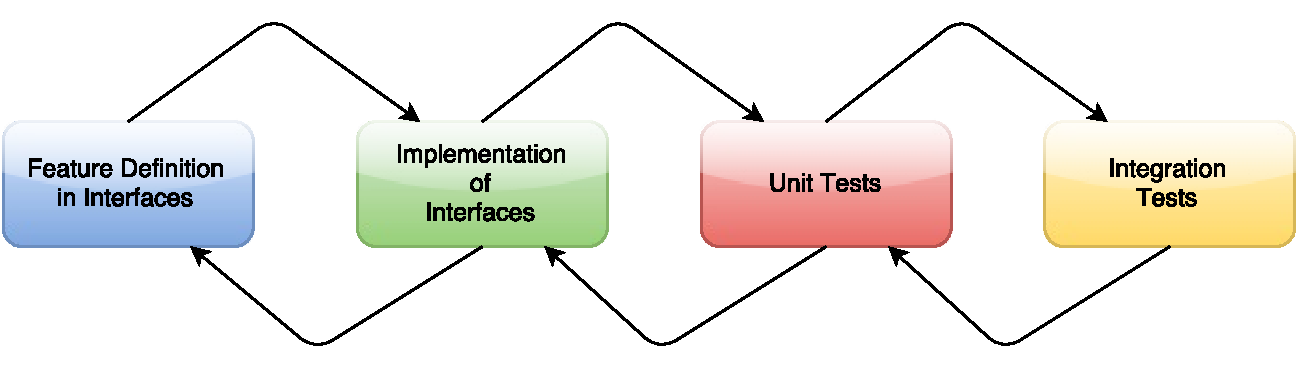
\includegraphics[scale=0.52]{images/work_process.pdf}
	\caption{Development Process}
	\label{development_process_of_a_feature}
\end{figure}

\begin{itemize}
	\item \textbf{Feature Definition in Interfaces}: We start by modelling the interfaces of our building blocks. While doing so, we try to be as compliant to the \textbf{Single Responsibility Principle} \footnote{objectmentor.com: Article on Single Responsibility Principle, see~\cite{singleresponsibility_objectmentor}} as possible. It helps by enforcing structures that are easy to reuse and change. However, we intentionally break it in some cases to allow more user-friendly interfaces (mostly in API entry-points).
	\\\\
	By defining the features in interfaces and writing logic against only them (instead of the direct implementations), we achieve complete independence between the implementing classes and are compliant to the \textbf{Open-Closed-Principle} \footnote{	objectmentor.com: Article on Open-Closed-Principle, see~\cite{openclosed_objectmentor}} internally ("Modules should be both open (for extension) and closed (for modification)" \footnote{Object-Oriented Software Construction, Prentice Hall, 1988, Bertrand Meyer, see~\cite{openclosed_bertrand}}). In combination with the Single Responsibility Principle this allows us to write more "pluggable" code.
	\item \textbf{Implementation of Interfaces}: Once the interfaces are properly defined, we write implementations for them according to the contracts set. As stated above, these classes are generally written against other interfaces internally instead of direct implementations.
	\item \textbf{Unit Tests}: Each feature must have a corresponding unit test. These are necessary to test each implementation for the right behaviour (outputs and side-effects) and stability for at least one given input. They also help to identify bugs in the implementations.
	\item \textbf{Integration Tests}: While Unit-Tests check the behaviour of every \textit{single} implementation, Integration Tests are used to cover the correct behaviour when used together with other parts of the project. With these tests we ensure all features interoperate properly with each other.
\end{itemize}
\noindent
Note that once a step is processed, that doesn't mean its result is final. As we can see in the diagram, we can go back and forth between the different steps at will to adapt to specific implementation problems and other new problems that have not been covered before.
\\\\
We choose this kind of on-the-fly structure because it suits the project best: We have to investigate different approaches before we can work out the real solution. Additionally, because "hibernate-search-engine" is an internal API, we have to be as flexible as possible with our development since some features of it can be different than what we might expect in the first place.
\\\\
It is worth mentioning that all the tests are executed during each build to ensure no regression bugs occur. This is automatically managed by the Maven \footnote{Maven project homepage, see~\cite{maven_homepage}} build tool.

\pagebreak
